\chapter{Results}

The fractal-like effect of the algorithm becomes more prominent when more iterations are applied.  The figure below shows the results at different numbers of iterations.  Starting with the simple case of applying a single iteration, the algorithm's way of working can easily be seen.  At one thousand iterations, the sphere begins to look like a planet.  Going beyond that with ten thousand iterations, the planet-like features are clearly exaggerated.

\fig{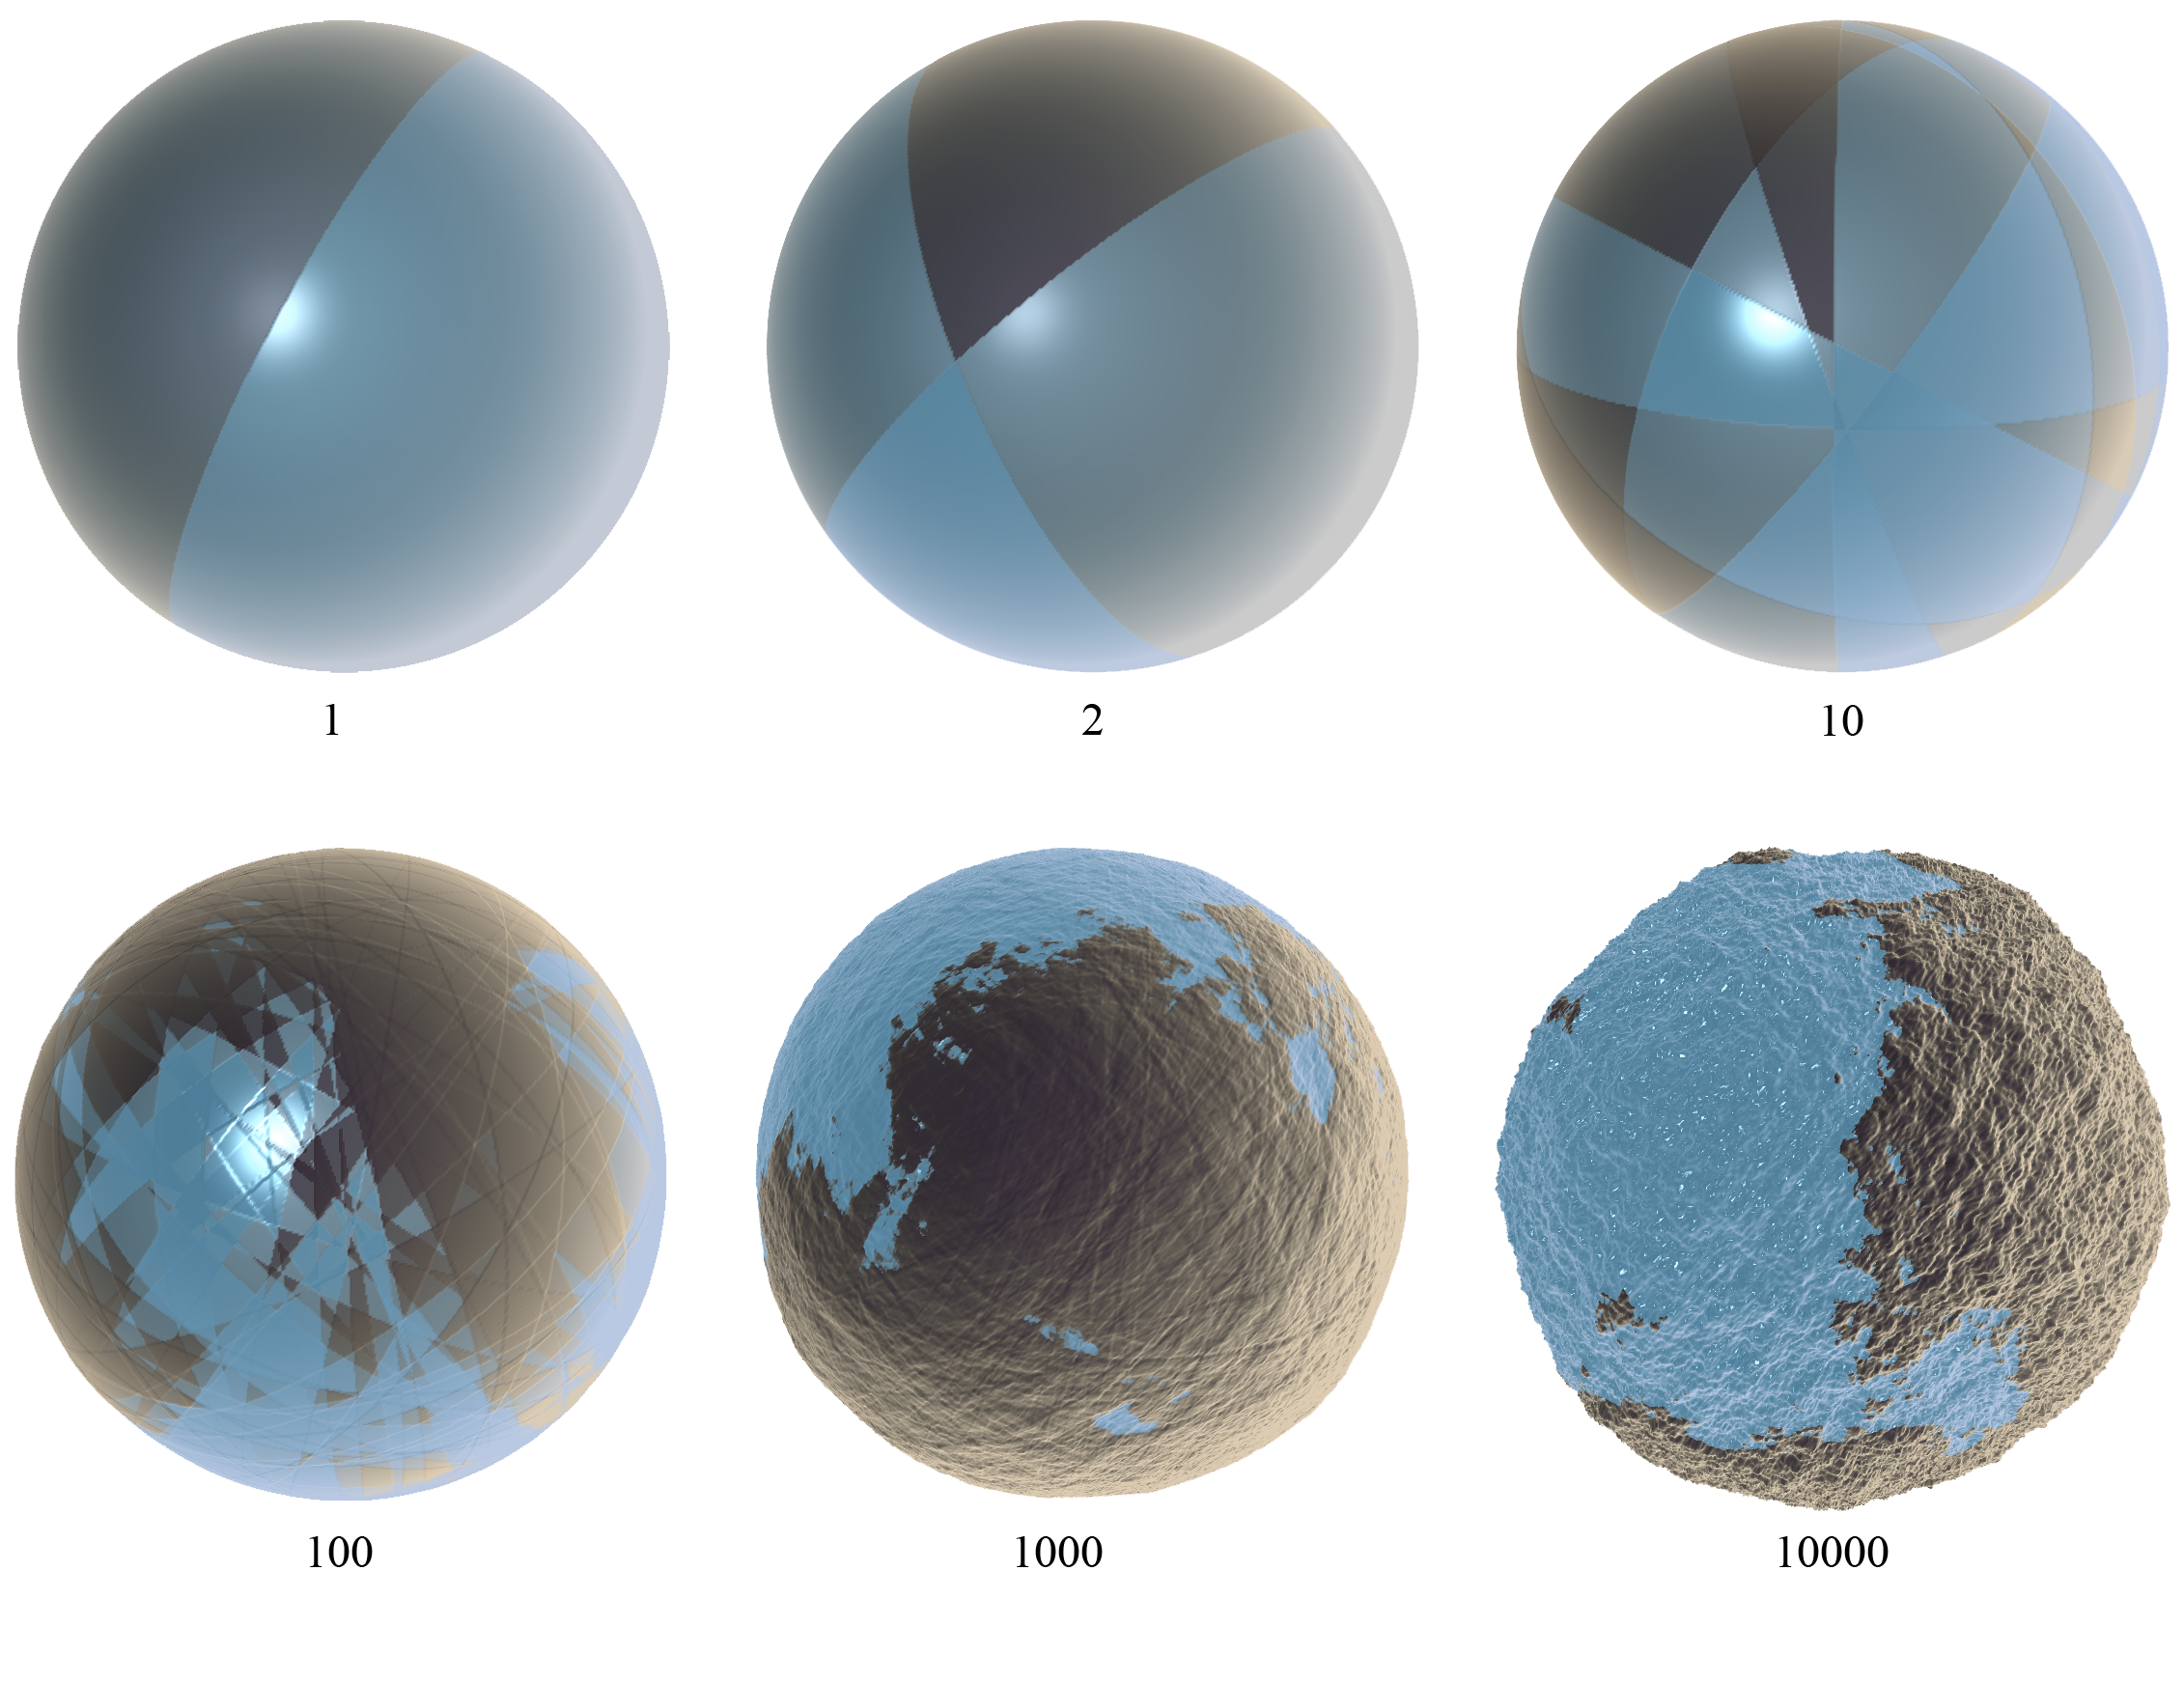
\includegraphics[width=0.9\textwidth]{iterations}}{The result of the algorithm applied with
  different numbers of iterations.}

A problem with the effects of the algorithm when modeling oceans is the fact that they become as
deformed as mountains.  The algorith does not discern between different types of surfaces on the
sphere.  Thus, modeling oceans requires a final step after applying the algorithm; smoothing out the
parts of the surface deemed to make up oceans.  This is trivially done by limiting the minimum
radius of each point on the sphere surface after applying all iterations.  Note that this cannot be
done continually between iterations; it would result in a biased distribution of the random
transformations, causing the sphere to start growing with each iteration.

A final example render of the algorithm is shown with exaggerated features for demonstrational
purposes.  The algorithm has been applied with $10000$ iterations, and two tweaks have been made to
it:

\begin{enumerate}
  \itemsep0em
  \item Splits were not done through the sphere center.
  \item Finally, water areas were smoothed out (with some noise).
\end{enumerate}

\noindent The image below was rendered with WebGL and a custom ambient-diffuse-specular material
fragment shader.

\fig{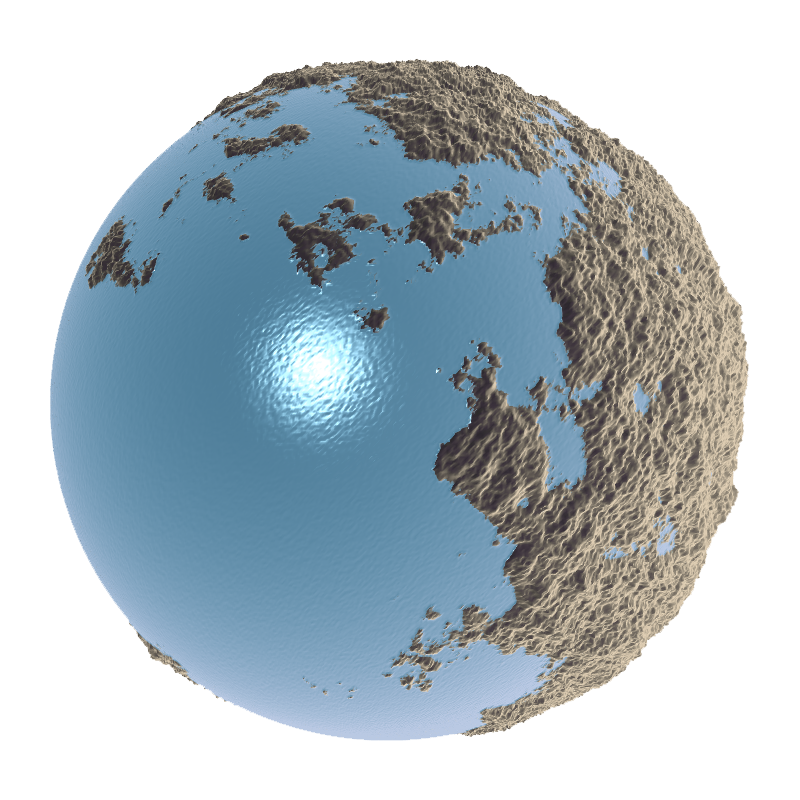
\includegraphics[width=0.8\textwidth]{final-render}}{Example render on a high-resolution sphere
  mesh.}
